\section{TESTING AND VALIDATION}
\subsection{Incremental testing}
To maintain coherence of the whole system, the project was implemented with a GIT workflow, this meant that each functionality was implemented in a separated branch and tested until working as the requirements specified.

When the functionality was implemented and tested, it was merged to the project.

\subsection{Sensor testing}

For the sensors, some public interfaces were used to test the correct functionality of the element:
\begin{itemize}
    \item Accelerometer: a public repository\cite{MMA8451driverMMA8451} with a class an a interface was used to the the correct reading of the acceleration values.
    \item Color sensor: as mentioned in the problems, a public project\cite{TCS3472_I2CClasswhich} was used to test the sensor and the interruption capabilities.
\end{itemize}

\subsection{\acrshort{i2c} validation}

To validate all the initialization of the sensors, the LHT00SU1 logical analyzer in \autoref{fig:osc} was used.
\begin{figure}[H]
    \centering
    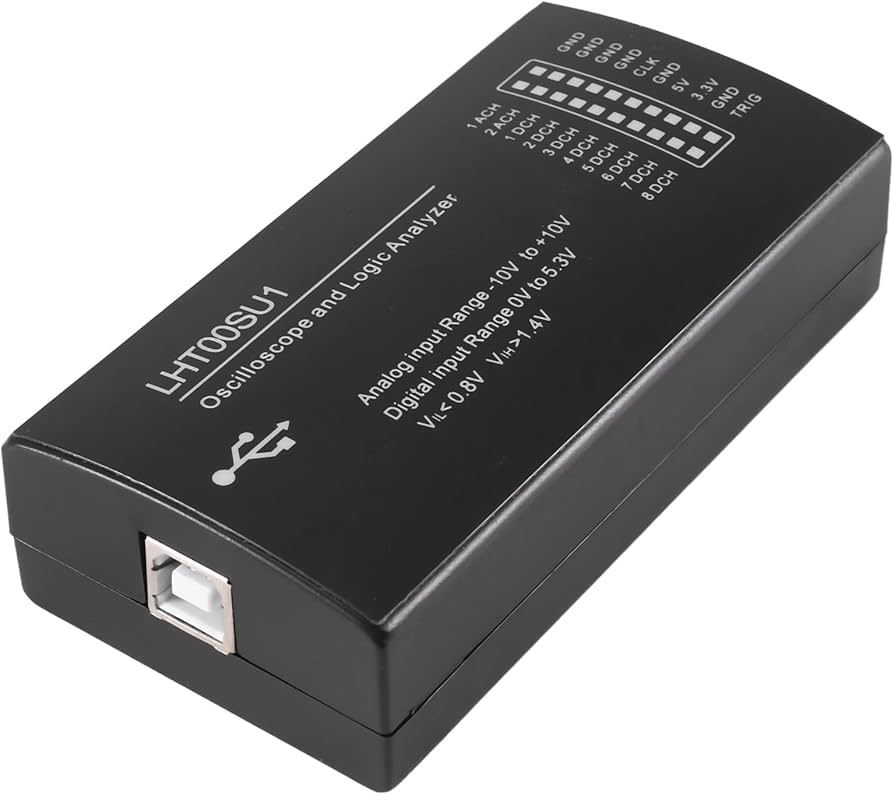
\includegraphics[width=0.4\textwidth]{images/7/Osc.jpg}
    \caption{Logical analyzer used in the project}
    \label{fig:osc}
\end{figure}

\subsection{Power mode validation}
To analyze the correct implementation of the power mode, the current going to the micro-usb connection of the L072CZ was characterized. The \autoref{fig:testCurrent} shows the current in the test mode and the \autoref{fig:AdvancedCurrent} shows the current in the advanced mode when 
the system is in sleep mode. 

Both pictures are done when the new state is waiting for the timeout. The only difference is that in the test mode picture, the led is turned on, so the current difference between them is less.
\begin{figure}[H]
    \centering
    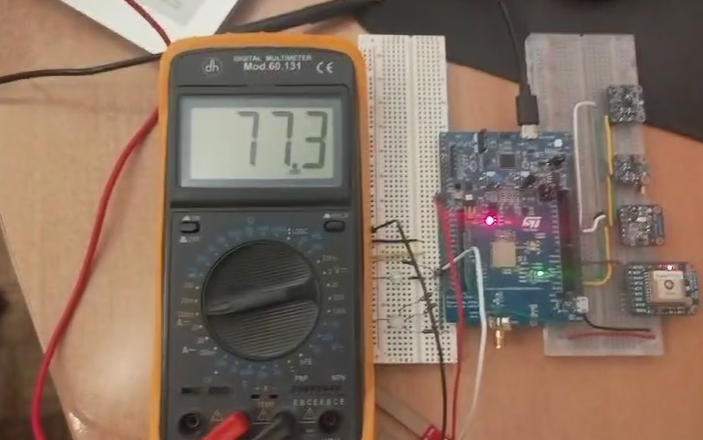
\includegraphics[width=0.7\textwidth]{images/7/Test2.png}
    \caption{Current in test mode}
    \label{fig:testCurrent}
\end{figure}
\begin{figure}[H]
    \centering
    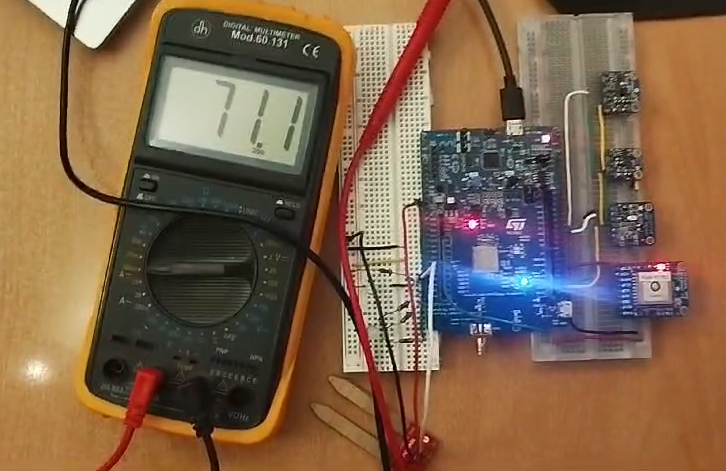
\includegraphics[width=0.7\textwidth]{images/7/Advanced.png}
    \caption{Current in the advanced mode}
    \label{fig:AdvancedCurrent}
\end{figure}